\documentclass[catalog.tex]{subfiles}

% do not write anything in the preamble
\begin{document}

\def\pbname{Fibonacci Heap} %change this, do not use any number, just the name

\section{\pbname} 

% only for overview, so short description (no more than 1-2 lines)
\begin{overview}
\item [Algorithm:] Construct and maintain a Fibonacci Heap
	% -	must match the label of the algorithm 
	% - when writing more than one algo use alg:\currfilebase_a, alg:\currfilebase_b, etc.
\item [Input:] one Fibonacci Heap
\item [Complexity:]$\mathcal{O}(\log n)$ for $extract\_min$ opearation and $\Theta(1)$ for other operations
\item [Data structure compatibility:] Fibonacci Heap
\item [Common applications:] Priority queue, Improvement for graph search algorithm like, Dijkstra Algorithm, A$^*$ Algorithm
\end{overview}


\begin{problem}{\pbname}
	Fibonacci heap is a data structure for priority queue operations. which is made up of a collection of rooted trees that are min-heap ordered. It has a better amortized running time than many other priority queues since most of the opearations in Fibonacci Heap take constant time.
\end{problem}

\subsection*{Description}
% Detailed description of the problem; More detailed information on the input and complexity; more applications with details on how they relate to each other (if this is the case). Do not hardcode references,  instead use the {\tt \textbackslash label} and {\tt \textbackslash reference} commands.  Examples: citation~\cite{ve477}, a group of figures (Fig.~\ref{fig:\currfilebase_group}), a sub-figure (Fig.~\ref{fig:\currfilebase_a}). To display a new line skip a line in the source code, do not use {\tt \textbackslash\textbackslash}.
\subsubsection*{Operations of a Fibonacci Heap}
Each element in a Fibonacci heap has a $key$. The heap supports the following seven opearations. ~\cite{intro3rd}
\begin{itemize}
	\item $Make\_heap()$ creates and then returns an empty new heap. \item $Insert(H,x)$ inserts an element $x$ into the heap $H$.
	\item $Minimum(H)$ returns a pointer to the element in $H$ with the minimum key.
	\item $Union(H_1,H_2)$ creates then returns a new heap that contains all elements of $H_1$ and $H_2$, with $H_1$,$H_2$ no longer used afterward.
	\item $Decrease\_key(H,x,k)$ assigns to element $x$ within $H$ a new key value $k$, where $k$ should be no greater than $x$'s current key value.
	\item $Delete(H,x)$ deletes element $x$ from $H$
\end{itemize}
\subsubsection*{Amortized time complexity}
\begin{table}[h]
	\centering
	\begin{tabular}{lc}
	Procedure     & Amortized time complexity \\ \hline
	Make\_heap    &   $\Theta(1)$                        \\
	Insert        &   $\Theta(1)$                        \\
	Extract\_min  &   $\mathcal{O}(\log n) $             \\
	Union         &   $\Theta(1)$                        \\
	Decrease\_key &   $\Theta(1)$                        \\
	Delete        &   $\mathcal{O}(\log n) $                      
	\end{tabular}
	\caption{Running times for operations onFibonacci heap. The number
	of items in the heap(s) at the time of an operation is denoted by n.}
	\label{tab:my-table}
	\end{table}
% add comment in the pseudocode: \cmt{comment}
% define a function name: \SetKwFunction{shortname}{Name of the function}
% use the defined function: \shortname{$variables$}
% use the keyword ``function'': \Fn{function name}, e.g. \Fn{\shortname{$var$}}
\subsection*{Structure of Fibonacci heaps}
An element in a Fibonacci heap has 7 atrributes. ~\cite{intro3rd} 
\begin{itemize}
	\item key: the key of the element.
	\item value: value stored in the element
	\item left: Pointer that points to the element's right siblings. If this element is an only child, its left is itself.
	\item right:  Pointer that points to the element's right siblings. If this element is an only child, its right is itself.
	\item parent:  Pointer thatpoints to the element's parent. For element in the root list of a Fibonacci heap, its parent is None. 
	\item child:  Pointer that points to one of its child. Its children are linked together in a circular, doubly linked list, which is called the child list of $x$.
	\item mark: A mark modified in $Decrease\_key$ and used in potential calculation.
\end{itemize}
\begin{figure}[h]
	\centering
	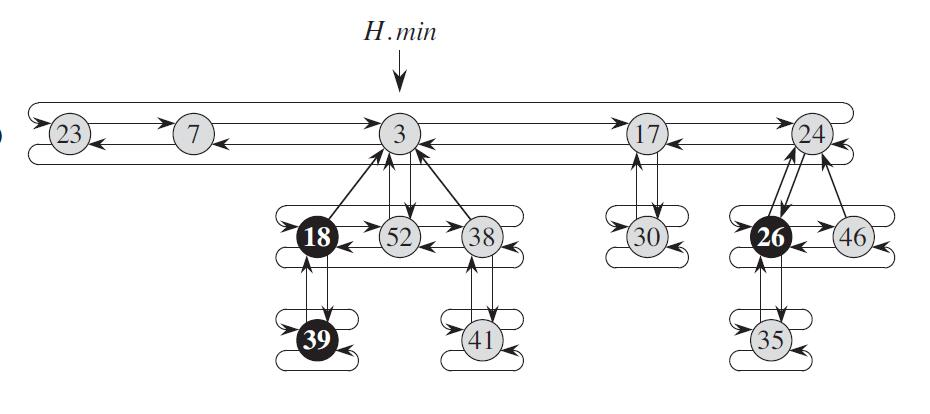
\includegraphics[width=0.7\textwidth]{problem-6.jpg}
	\caption{An example of a Fibonacci heap}
\end{figure}
\subsubsection*{Make an empty heap}
Make an empty heap $H$ is to set the $H.min$ to be None and the current size of $H$ to be 0.  
\newpage
\subsubsection*{Insert a node}
\par When a node is to be inserted, it is assumed to have already been allocated with its key already set.
\begin{Algorithm}[Insert($x$)\label{alg:\currfilebase_insert}]
	% -	must match the reference in the overview
	% - when writing more than one algo use alg:\currfilebase_a, alg:\currfilebase_b, etc.
	% \SetKwFunction{myfunction}{Consolidate}	
	\Input{A node $x$ to be inserted}
	\Output{The minimum element in $H$ and modified $H$}
	$x.degree=0$ \\
	$x.parent=None$ \\
	$x.child=None$ \\
	$x.mark=False$ \\
	\If{H.min==None}{
		create a root list for $H$ with just x \\
		$H.min=x$
	}
	\Else{
		insert $x$ into $H$'s root list \\
		\If {$x.key<H.min.key$}{
			$H.min=x$
		}
	}
	$H.size +=1$
		% \Fn{\myfunction{$H$}}{
		% }
\end{Algorithm}
\subsubsection*{Union two Fibonacci heaps}
\par When uniting two Fibonacci heaps into one new Fibonacci heap, the things to do are simply concatenating the root lists of both Fibonacci heaps and then determining the new minimum node. After such union operations, the old two Fibonacci heaps will not be used any more. 
\begin{Algorithm}[Union($H_1,H_2$)\label{alg:\currfilebase_union}]
	% -	must match the reference in the overview
	% - when writing more than one algo use alg:\currfilebase_a, alg:\currfilebase_b, etc.
	% \SetKwFunction{myfunction}{Consolidate}	
	\Input{Fibonacci heap$H_1,H_2$ }
	\Output{A new Fibonacci heap $H$, which is the union heap}
	$H=make_heap()$ \\
	$H.min=H_1.min$ \\
	concatenate the root list of $H_2$ with the root list of $H$ \\
	\If{$H_1.min==None$ or $(H_2.min \neq None$ and $H_2.min,key<H_1.min.key)$ }{
		$H.min=H_2.min$
	}
	$H.size=H_1.size+H_2.size$ \\
	\Ret $H$
\end{Algorithm}
\newpage
\subsubsection*{Extract the minimum node}
\par This process is the most complicated opearations of a Fibonacci heap. It is where the maintainence of heap property and the work of consolidating trees in the root list occurs.
\begin{Algorithm}[Extrcact\_min($H$)\label{alg:\currfilebase_extract}]
	% -	must match the reference in the overview
	% - when writing more than one algo use alg:\currfilebase_a, alg:\currfilebase_b, etc.
	\Input{Fibonacci Heap $H$}
	\Output{The minimum element in $H$ and modified $H$}
	$z=H.min$ \\
	\If{$z \neq None$}{
		\For{each child of $z$}{
			add $x$ to the root list of $H$ \\
			$x.p = None$
		}
	}
	remove $z$ from the root list of $H$
	\If{$z==z.right$}{
		$H.min=None$
	}
	\Else{
		$H.min=z.right$ \\
		$Consolidate(H)$
	}
	$H.size-=1$ \\
	\Ret z

\end{Algorithm}
\par The upper bound $D(n$) on the degree of any node in an n-node Fibonacci heap meets that 
$$
D(n) \leq \lfloor \log_{\phi}n \rfloor
$$
where $\phi$ is the golden ratio, defined as
$$
\phi = \frac{\sqrt{5}+1}{2}
$$
\begin{Algorithm}[Consolidate($H$)\label{alg:\currfilebase_cons}]
	\SetKwFunction{myhl}{Heap\_link}
	\Fn{\myhl{}}{
		remove $y$ from the root list of $H$ \\
		make $y$ a child of $x$ \\
		incrementing $x.degree$ \\
		$y.mark=FALSE$
	}
	
	let $A$ be a new array with size D(n) \\
	Set each element of $A$ $None$ \\
	\For{each node $w$ in the root list of $H$}{
		$x=w$ \\
		$d=x.degree$ \\
		\While{$A[d] \neq None$}{
			$y=A[d]$
			\If{$x.key>y.key$}{
				exchange $x$ with $y$
			}
			\myhl{$y,x$} \\
			$A[d]=None$
			$d=d+1$
		}
		$A[d]=x$
	}
	$H.min=None$ \\
	\For{every element $i$ in $A$}{
		\If{$A[i] \neq None$}{
			\If{$H.min==None$}{
				create a new root list of $H$ that only contains $i$ \\
				$H.min=i$
			}
			\Else{
				insert $i$ into $H$ root list \\
				\If{$i.key < H.min.key$}{
					H.min=i
				}
			}
		}
	}
\end{Algorithm}
\newpage
\subsubsection*{Decrease a key and delete a node}
$Decrease\_key$ opearation decreases the key of one certain node. All of such operations are done under the assumption that removing a node from a linked list won't change any of its structural atrributes.
\begin{Algorithm}[Decrease\_key($x,k$)\label{alg:\currfilebase_dec_k}]
	\SetKwFunction{mycut}{Cut}	
	\SetKwFunction{mycascut}{Cascading\_cut}
	\Input{The target node $x$, the value to decrease $k$ }
	\Output{Nothing}
	\Fn{\mycut{$H,x,y$}}{
		remove $x$ from the child list of $ y $\\
		$y.degree-=1$\\
		add $x$ to the root list of $H$ \\
		$x.parent=Null$ \\
		$x.mark=false$
	}
	\Fn{\mycascut{$H,y$}}{
		$z=y.parent$ \\
		\If{$z \neq None$}{
			\If{$y.mark==false$}{
				$y.mark==true$
			}
			\Else{
				\mycut{$H,y,z$}\\
				\mycascut{$H,z$}
			}
		}
	}
	\If{$k>x.key$}{
		this causes error.
	}
	\BlankLine
	$x.key=k$ \\
	$y=x.parent$ \\ 
	\If{$y \neq None$ and $x.key<y.key$}{
		\mycut{$H,x,y$} \\
		\mycascut{$H,y$}
	}
	\If{$x.key<H.min.key$}{
		$H.min=x$
	}
\end{Algorithm}
\par What $Delete$ does is decrease the key of the element to be deleted and call $Extract\_min$. Assume that there is no key value of $-\infty$ currently
in the Fibonacci heap.
\par There is a question that in pratical use we cannot actually find the address of or the pointer itself. The first solution I think is Ostrich Algorithm, that the probability of having to delete another element besides the minimum within the heap is very small since we have already decided to use Fibonacci heap rather than other heaps. A more relatively solution is to set up a dictionary for the Fibonacci heap, where the key of the dictionary is the value of all elements, the value of the dictionary is the element or the address of the element. So we can delete an element by its value.

\begin{Algorithm}[Delete($H,x$)\label{alg:\currfilebase_union}]
	% -	must match the reference in the overview
	% - when writing more than one algo use alg:\currfilebase_a, alg:\currfilebase_b, etc.
	% \SetKwFunction{myfunction}{Consolidate}	
	\Input{Fibonacci heap$H$, the element to be deleted $x$ }
	\Output{Nothing}
	$Decrease\_key(H,x,-\infty)$ \\
	$Extract\_min(H)$
\end{Algorithm}

% include references where to find information on the given problem using latex bibliography
% insert references in the text (\cite{}) and write bibliography file in problem-nb.bib (replace nb with the problem number)
% prefer books, research articles, or internet sources that are likely to remain available over time
% as much as possible offer several options, including at least one which provide a detailed study of the problem
% if available include links to programs/code solving the problem
% wikipedia is NOT acceptable as a unique reference

$\ $
\newpage
\subsubsection*{Amortized Analysis}
\begin{enumerate}
	\item Notations and the potential function.
	The notations used in analysis is shown in the table below. \\
	\begin{table}[h]
		\centering
		\begin{tabular}{cc}
		notation     & meaning                          \\ \hline
		n            & number                           \\
		rank(x)      & number of children of node x     \\
		Extract\_min & max rank of any node in heap H   \\
		trees(H)     & number of trees in heap H        \\
		marks(H)     & number of marked nodes in heap H
		\end{tabular}
		\caption{Notations in amortized analysis}
		\label{notation}
	\end{table}
	\par The potential function is ~\cite{ve281}
	$$
	\Phi(H)=\operatorname{trees}(H)+2 \cdot \operatorname{marks}(H)
	$$
	\item $Insert$: \\
	The actual cost is $c_i=\mathcal{O}(1)$. Change in potential is $\Delta \Phi = 1$. The amortized cost is calculated as $\hat{c}_{i}=c_{i}+\Delta \Phi=\Theta(1)$.
	\item $Extract\_min$: \\
	The actual cost is $c_{i}=\mathcal{O}({rank}(H))+\mathcal{O}({trees}(H))$. Change in potential is $\Delta \Phi \leq \operatorname{rank}\left(H^{\prime}\right)+1-\operatorname{trees}(H)$.\\
	The amortized cost is calculated as $\hat{c}_{i}=c_{i}+\Delta \Phi=\mathcal{O}(r a n k(H))+\mathcal{O}\left(r a n k\left(H^{\prime}\right)\right)=\mathcal{O}(\log n)$, where the rank of heap with size $n$ is $\mathcal{O}(\log n)$.
	\item $Decrease\_key$: \\
	The actual cost $c_{i}=\mathcal{O}(c)$, where c is the number of cuts. Change in potential is $\Delta \Phi \leq c+2 \cdot (-c+2) = \mathcal{O}(1)-c$. \\
	The amortized cost is calculated as $\hat{c}_{i}=c_{i}+\Delta \Phi=\mathcal{O}(1)$
\end{enumerate}
\singlespacing
\newpage
\printbibliography[title={References.},resetnumbers=true,heading=subbibliography]

\end{document}
